\documentclass{article}
\usepackage{tikzinclude, pgfplots}
\usetikzlibrary{positioning}

\title{Using tikz}
\author{Arctan}
\date{Dec 22}

\pgfplotsset{compat=1.18}
\begin{document}
\maketitle

\section{Tikz}
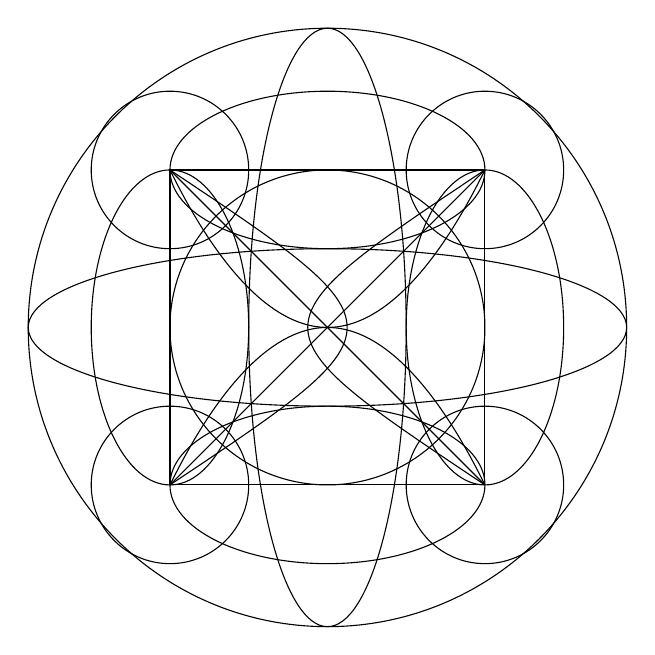
\begin{tikzpicture}
    \draw (0,0) -- (4,0) -- (4,4) -- (0,4) -- cycle;
    \draw (0,0) -- (4,4);
    \draw (0,4) -- (4,0);

    \draw (0,0) circle (1);
    \draw (4,4) circle (1);
    \draw (0,4) circle (1);
    \draw (4,0) circle (1);

    \draw (2,2) circle (2);

    % \draw (0,0) parabola (6,2);
    \draw (0,0) parabola bend (2,2) (4,0);    
    \draw (0,4) parabola bend (2,2) (4,4);    

    % \draw (0,0) parabola bend (2,2)  (0,4);   
    % \draw (4,0) parabola bend (2,2)  (4,4); 

    \draw (0,0) .. controls (3,2) .. (0,4);
    \draw (4,0) .. controls (1,2) .. (4,4);

    
    \draw (2,4) ellipse (2 and 1);
    \draw (2,0) ellipse (2 and 1);
    \draw (4,2) ellipse (1 and 2);
    \draw (0,2) ellipse (1 and 2);

    \draw (2,2) circle (3.8);

    \draw (2,2) ellipse (3.8 and 1);
    \draw (2,2) ellipse (1 and 3.8);

\end{tikzpicture}
\vspace{0.5in}

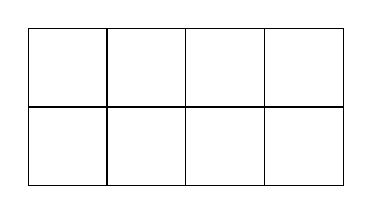
\begin{tikzpicture}
    \draw (0,0) grid (4,2);
\end{tikzpicture}

\newpage
\section{More tikz}
\begin{center}
    
\begin{tikzpicture}[transform canvas={scale=4.0}]
       \draw[blue] (0,1) arc (90: -90:0.5cm and 1cm);
       \draw[dashed, red] (0,1) arc (90:270:0.5cm and 1cm);
       \draw (0,0) circle (1cm);
       \filldraw[red] (0,1) circle (0.05cm);
       \filldraw[red] (0,-1) circle (0.05cm);
       \shade[ball color=blue!20!white, opacity=0.3] (0,0) circle (1); %20% blue and 80% white
    \end{tikzpicture}
\end{center}

\newpage
\section{Lines and nodes}
\begin{center}
    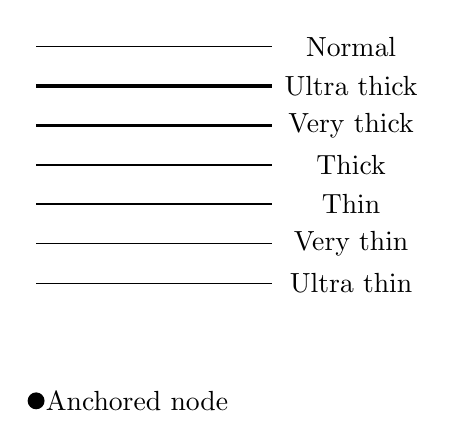
\begin{tikzpicture}
        \draw (0, 0.5) -- (3, 0.5);
        \draw[ultra thick] (0,0) -- (3,0);
        \draw[very thick] (0,-0.5) -- (3,-0.5);
        \draw[thick] (0,-1) -- (3,-1);
        \draw[thin] (0,-1.5) -- (3,-1.5);
        \draw[very thin] (0,-2) -- (3,-2);
        \draw[ultra thin] (0,-2.5) -- (3,-2.5);

        \draw node at (4, 0.5) {Normal};
        \draw node at (4, 0) {Ultra thick};
        \draw node at (4, -0.5) {Very thick};
        \draw node at (4, -1) {Thick};
        \draw node at (4, -1.5) {Thin};
        \draw node at (4, -2) {Very thin};
        \draw node at (4, -2.5) {Ultra thin};

        \filldraw (0, -4) circle (0.1cm) node[anchor=west]{Anchored node};
    \end{tikzpicture}
\end{center}

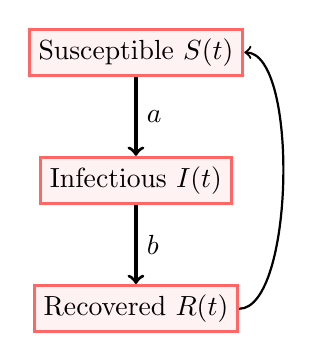
\begin{tikzpicture}[
    SIR/.style={rectangle, draw=red!60, fill=red!5, very thick, minimum size=5mm},  
]
    % Nodes
    \node[SIR] (Sus)    {Susceptible $S(t)$};
    \node[SIR] (Inf) [below= of Sus] {Infectious $I(t)$};
    \node[SIR] (Rec) [below= of Inf] {Recovered $R(t)$};

    % Lines
    \draw[->, very thick] (Sus.south) to node[right] {$a$} (Inf.north);
    \draw[->, very thick] (Inf.south) to node[right] {$b$} (Rec.north);
    \draw[->, thick] (Rec.east) .. controls +(right:7mm) and +(right:7mm) .. (Sus.east);
\end{tikzpicture}

\newpage
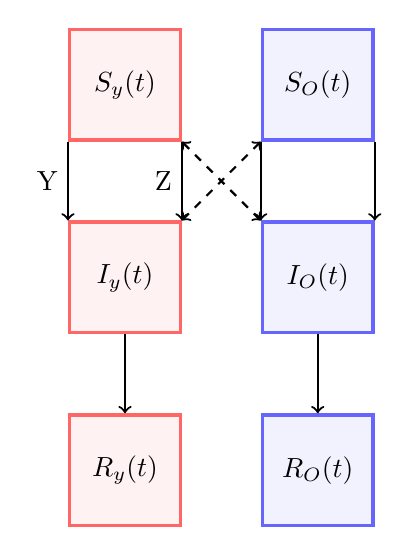
\begin{tikzpicture}[
    yn/.style={rectangle, draw=red!60, fill=red!5, very thick, minimum size=40},
    on/.style={rectangle, draw=blue!60, fill=blue!5, very thick, minimum size=40},
]
    % Nodes
    \node[on] (Suss)    {$S_O(t)$};
    \node[on] (Inff)  [below= of Suss]    {$I_O(t)$};
    \node[on] (Recc)  [below= of Inff]    {$R_O(t)$};

    \node[yn] (Susy) [left = of Suss]   {$S_y(t)$};
    \node[yn] (Infy) [left= of Inff] {$I_y(t)$};
    \node[yn] (Recy) [left= of Recc] {$R_y(t)$};

    % Lines

    \draw[->, thick] (Susy.south west) to node[left] {Y} (Infy.north west);
    \draw[->, thick] (Susy.south east) to node[left] {Z} (Infy.north east);

    \draw[<->, dashed, thick] (Susy.south east) to node[left] {} (Inff.north west);
    \draw[<->, dashed, thick] (Suss.south west) to node[left] {} (Infy.north east);
    
    \draw[->, thick] (Suss.south west) to node[left] {} (Inff.north west);
    \draw[->, thick] (Suss.south east) to node[left] {} (Inff.north east);

    \draw[->, thick] (Infy.south) to node[left] {} (Recy.north);
    \draw[->, thick] (Inff.south) to node[left] {} (Recc.north);

    

\end{tikzpicture}

\end{document}